\documentclass{article}
\usepackage[utf8]{inputenc}
\usepackage{tikz} %package for plots, graphics and functions

\title{01 Drawing Lines}
\author{Arman Daneshdoost}
\date{March 2024}

\begin{document}
	\maketitle
	\begin{figure}[h]
	\centering
	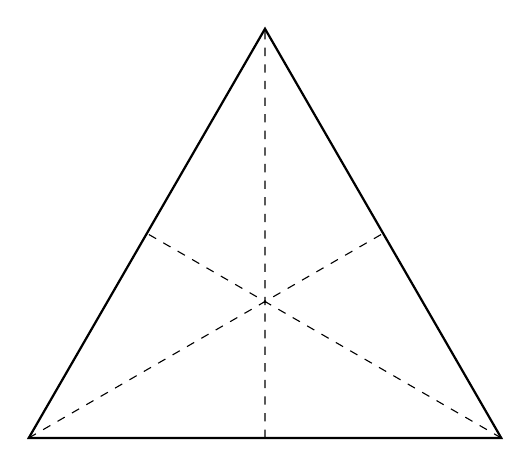
\begin{tikzpicture}[scale = 3] % you can add xscale and yscale : [xscale = ..., yscale=...]
		\draw[thick] (0,0) -- (2,0 )-- (1, {sqrt(3)}) -- cycle ; % cycle means to returning to first point (0,0) - you can specify line weight [thick]
		\draw [dashed] (1,0) -- (1, 1.73205) (0,0) -- (1.5, 0.866) (2,0) --(0.5, 0.866); %Three medians of triangle
	\end{tikzpicture}
	\caption{My sweet triangle}
	\end{figure}
	\begin{tikzpicture}[scale = 2]
		\draw (0,1) -- (0, -1) -- (2,0) -- cycle;
		\draw (0,0) -- (2,0);
	\end{tikzpicture}
\end{document}